\documentclass[sigconf]{acmart}

\usepackage{booktabs} % For formal tables
\usepackage{multirow}

% Copyright
%\setcopyright{none}
%\setcopyright{acmcopyright}
%\setcopyright{acmlicensed}
\setcopyright{rightsretained}
%\setcopyright{usgov}
%\setcopyright{usgovmixed}
%\setcopyright{cagov}
%\setcopyright{cagovmixed}


%%Conference
\acmConference[CASES 2017]{International Conference on Compilers, Architecture,
and Synthesis for Embedded Systems}{October 2017}{Seoul, South Korea} 
\acmYear{2017}
\copyrightyear{2017}

\begin{document}
\title{Read Only Data Specific Management for an Energy Efficient Memory System}
\titlenote{Produces the permission block, and
  copyright information}


\author{Gregory Vaumourin, Alexandre Guerre, Thomas Dombek}
\affiliation{
  \institution{CEA LIST}
  \city{Gif sur Yvette} 
  \state{France} 
  \postcode{F-91191}
}
\email{{firstname}.{lastname}@cea.fr}


\author{Denis Barthou}
\affiliation{%
  \institution{INRIA Bordeaux Sud-Ouest, LaBRI}
  \streetaddress{Institute of Technology}
  \city{Bordeaux} 
  \state{France} 
%  \postcode{43017-6221}
}
\email{denis.barthou@inria.fr}


\begin{abstract}
Traditional cache-based memory hierarchies, especially in the context of embedded systems, present many challenges in power consumption and scalability. With the end of the CMOS scalability, one way to increase the energy efficiency of the cache hierarchy is to propose heterogeneous data management inside caches. The L1 level caches are usually divided between instructions and data, notably because of their differences in data locality of the stream. Based on a previous study, we propose to go further in this direction by proposing dedicated cache structures for read-only data for two reasons: locality improvement and coherence optimization. Several architectural options are explored where we designed a dedicated data path for read-only data. We proposed a static analysis at compile-time to perform the detection of read-only data at cache block granularity. This classification presents a detection rate of 89.3\% in average when compared to an offline analysis. Evaluated with Gem5 and McPat in a multicore environment with a set of multithreaded image processing benchmarks, the new memory organization with a shared read-only L1-level cache shows an average of 16.7\% of energy savings without any loss in performance. 
\end{abstract}

%
% The code below should be generated by the tool at
% http://dl.acm.org/ccs.cfm
% Please copy and paste the code instead of the example below. 
%

% \begin{CCSXML}
%<ccs2012>
%<concept>
%<concept_id>10010520.10010521.10010528.10010536</concept_id>
%<concept_desc>Computer systems organization~Multicore architectures</concept_desc>
%<concept_significance>500</concept_significance>
%</concept>
%</ccs2012>
%\end{CCSXML}

%\ccsdesc[500]{Computer systems organization~Multicore architectures}
%\ccsdesc[500]{Computer systems organization~Embedded systems}

\keywords{Cache memory, read-only, data locality}


\maketitle

\section{Introduction}

Caches are widely used in modern processors to effectively hide the data access latency. But with the number of cores increasing, the use of hardware-controlled caches increases the energy consumption for two reasons. The automatic data management in caches is costly and coherence protocols typically do not scale very well with the number of cores. The cache hierarchy consumes between 25\% and 50\% of the energy of the chip~\cite{Segars:2001} on current systems. With the growing focus on energy efficiency, it is important to find ways to reduce energy without sacrificing performance. Usually the memory stream is handled in an uniform way by the memory system that has limited knowledge about the context of data being loaded. Heterogeneous management classifies data or accesses into several types in order to isolate and take advantage of the potential that exist in sub-sets of the memory stream. In the state of the art, such techniques are used for two reasons: locality and coherence optimization.  

There has been a number of previous works that attempts to classify data based on locality~\cite{Gonzalez:1995,Kang:2011,Lee:2000,Geiger:2005} . Access patterns to instructions, the heap, the stack and even global data items show a variety of different reuse patterns so that specific cache structures can be build for each type. This type of solution has been studied with success since the early days of cache memories. In the 60s, Harvard architectures separate the L1-level cache into instruction and data cache. Since the 90s, many solutions have been proposed~\cite{Gonzalez:1995,Kang:2011,Lee:2000,Geiger:2005} to enhance this type of solution with dedicated cache memories for specific type of data (stack cache, ...). They bring important dynamic energy consumption reduction if the separation of data results in two sub-groups of data with very different locality properties. The difficulty of such proposition is to perform the data classification at hardware-level and drive the request to the relevant sub-memory. 


Heterogeneous management has also been proposed for coherence cost reduction. Indeed, classification of data into private and shared has proven to be an efficient solution in this case since private data can be taken out of coherence and resources can be concentrated on providing coherence solely for shared data. This is based on the observation that few memory blocks actually require coherence, only 18\% of the OS pages are in Shared Read-Write state on PARSEC on average~\cite{Cuesta:2013}. It allows to simplify coherence in multicore architectures by reducing its associated costs (area, energy, performance) and therefore increasing scalability. Most of the solutions perform the classification in a reactive fashion during the execution at an OS-page granularity. 


We propose in this paper the specific management of read-only data as an approach in the middle of both groups of solutions. In this paper, read-only is studied as a dynamic property over time, so data can exist in a read-only state for a specific amount of time. We study the benefit of a specific read-only data management for both locality and coherence optimization. The coherence potential is simple as read-only data can simply be taken out of the coherence tracking. The locality potential is less intuitive but has been illustrated in a previous embedded system study~\cite{vaumourin:2014}. This work has shown a high locality potential of a heterogeneous management of read-only data, especially for image processing applications due to their implementation as a pipeline of tasks.

The contributions of the paper are the following:
\begin{itemize}
\item An illustration of the difference of behavior between read-only and read-write data
\item A light-weight efficient data classification scheme at compile time
\item A full hardware/software codesign solution with and an architectural exploration for the specific management of the read-only data in the cache hierarchy. 
\end{itemize}

The experimental evaluation shows that our proposed solution decreases the energy consumption of the memory system by 16.7\% on average without a performance penalty on a representative set of multithreaded image processing benchmarks. The data classification scheme performed at compile-time, achieves a detection rate of 89.3\% in average compared to an offline analysis technique. Removing the coherence tracking of the dedicated RO datapath allows to decrease the network traffic by 26.0\% 

The organization of this paper is the following: Section 2 discusses the related work, Section 3 illustrates the locality difference of read-only data. Section 4 details the compile-time data classification scheme. Section 5 highlights our architecture exploration methodology and the evaluation methodology. Section 6 describes the experiments results. Section 7 studies a specific optimization for the read-only datapath. Finally, Section 8 provides our conclusions.

\section{Related Work}

As mentioned before, the specific management in the memory system based on based on data classification has been successfully studied in the past. These solutions creates two (or more) sub-groups of data with different properties that can be exploited separately. The problems encoutered with such solutions are the efficiency of the classification scheme . We focus on heterogenous data management solutions that optimize for locality and coherence. 

\subsection{Locality Optimization} 

Apart from the locality principle, the locality properties are far from being uniform accross the working set and differences can be exploited. This difference is often intuitive like the difference between data and instructions. Instructions represent a very small part working set that it is accessed much more than other data, which is one of the justification of a separation at the first level between instruction and data cache. Going further in this direction, Gonzales \textit{et al.}\cite{Gonzalez:1995} first proposed L1 data cache with separate sub-structures one for data with high temporal locality (temporal cache) and one for high spatial locality data (spatial cache) that has been improved by Adamo \textit{et al.}\cite{Adamo:2009}. This is based on the observation that most data present either spatial locality such as arrays or temporal locality such as stack data, few data have both temporal and spatial locality at the same time. The classification focuses on detecting whether the accessed data is part of an array to place them in the spatial cache. In order to achieve that, the solution includes a history table that detects strided accesses that are predicted to belong an array. Having separated structures allows to optimize further the cache design and in this case, the temporal and spatial sub-caches have different blocksizes and replacement policies. Lee \textit{et al.}\cite{Lee:2000} propose to divide the data cache into separate structures for stack, heap, and global data. Geiger goes further by splitting the heap cache into 2 sub-parts~\cite{Geiger:2005}. Those solutions rely on being able to distinguish data types based solely on the address, possibly with some system support. Without operating system and hardware support, these approaches will not work when Address Space Layout Randomization (ASLR) is used for security, because these techniques involve randomly relocating the program stack, heap, and shared libraries at runtime. Kang \textit{et al.}\cite{Kang:2011} proposed a stack cache that is able to detect stack data accesses by determining whether the address is an offset from the stack pointer register. Those solutions are often more effective at reducing the miss rate compared to a naive cache size augmentation while being more energy efficient. The main drawbacks of such technique are the classification mechanism that stays quite simple and at hardware-level. Also, none of those solutions makes distinctions based on read/write access patterns of data. As the locality difference between RW and RO data is not obvious, it already been studied been illustrated in a previous study \cite{vaumourin:2014} and an extension of this analysis is presented farther in this paper, which justify the specific read-only data management for locality purpose. 

\subsection{Coherence Optimization}

A common approach is the classification of data into private and shared\cite{Ros:2012,Cuesta:2013, Davari:2015,Hardavellas:2009,Pugsley:2010,Hossain:2011} resulting in directory size reduction, or optimizing the coherence protocol itself by replacing explicit coherence invalidations with silent self-invalidation of shared data~\cite{Ros:2012}. The OS approach is the most common for such optimization because it does not impose extra requirements for dedicated hardware, since data classification at page granularity is stored along with the page table entries (PTEs)~\cite{Hardavellas:2009}. This makes a good choice for complexity-effective optimizations. These solutions mostly detect read-only data at page granularity in a reactive fashion. A page is first considered read-only and a single write on the page switches the status of the page into read-write mode. Compared to a block granularity detection, page granularity can produce poor detection rates and leads to under-optimal solutions. On the evaluated applications in \cite{Cuesta:2013}, the detection rate of read-only data goes from under 40\% to more than 60\% when switching from page to block granularity. Moreover, hardware-based proposition are area-constrained and limited to simple detection methods such as saturation counters. 

Although incurring minimum hardware cost, compiler-driven classification is not transparent to software as it needs recompilation. It is well suited for hardware/software co-design, but requires significant effort to determine at compile time if a variable is going to be shared or not. The only work in that direction is from Kim \textit{et al.}\cite{Kim:2010}. Proving the sharing state of a data is hard at compile level, so the analysis allows classication error in order to increase the proportion of detected shared data. However, it has to rely on hardware mechanisms to recover from those errors. Also, the classification is static so variable do not change states during execution. The RO/RW classification in such optimizations is seen as an extension on top of the private/shared classication. Also, they usually do not propose specific strutures to store the shared data that would allow to optimize for locality and cache ressource as well. An exception to this is the solution of Cebrian \textit{et al.}\cite{cebrian:2017} that proposes a dedicated shared L1 cache that is logically shared but physically distributed accross all cores. This solution shows an important miss reduction at L1-level, however it does not scale very well as remotely accessing a cache line in the shared cache can be as expensive as a miss in the L2 cache. 

As seen in the previous solutions, an efficient classification scheme is a key point for achieving a good solution for heterogeneous management. The next section discusses the locality difference between RO and RW data.

\section{Read-only Data Characterization}


We define read-only data as data used in a read mode either for the whole application execution (input data) or for a more limited scope such as a function, a kernel or a loop. In this case, read-write data can switch into read-only mode for some scope and then switch back to read-write mode. Our analysis is mostly focused on image processing applications, since these applications are often implemented as a pipeline of tasks where the output (written) data of a task corresponds to the input (read) data of the next one. Such computations manipulate large regions that are in a read mode on a long scope.

\begin{figure}
    \centering
    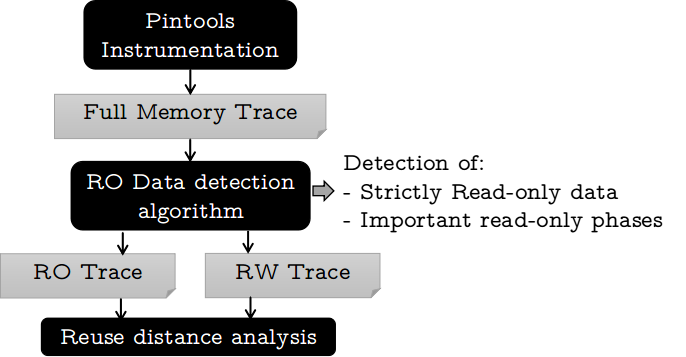
\includegraphics[width=9cm]{./images/localityworkflow.png}
     \caption{Workflow of the locality Analysis}
    \label{localityworkflow}
\end{figure}
We study the separation of the memory stream with a data locality metric: the reuse distance~\cite{Coffman:1973}. This metric is defined as the number of different accesses between two accesses to the same address and depends only on the cache block size (fixed to 64B). A two-step analysis described \ref{localityworkflow} is followed: First, a memory trace is extracted from an instrumented execution of the analyzed application. Then, the read-only data and read-only periods are detected through an analysis of the memory trace. This offline analysis explores the trace in a 2D space (time and address) to detect rectangular areas solely composed of read accesses. Such analysis is manually tuned to detect read areas in an adequate grain in order to avoid capturing every read access as a small read-only area. The main memory trace is then split in read-only and in read-write traces. The average reuse distance is computed on all traces: The original trace and the 2 sub-traces. The results, shown in Figure \ref{stackdistance}, are normalized to the average reuse distance of the full trace.


\begin{figure}
    \centering
    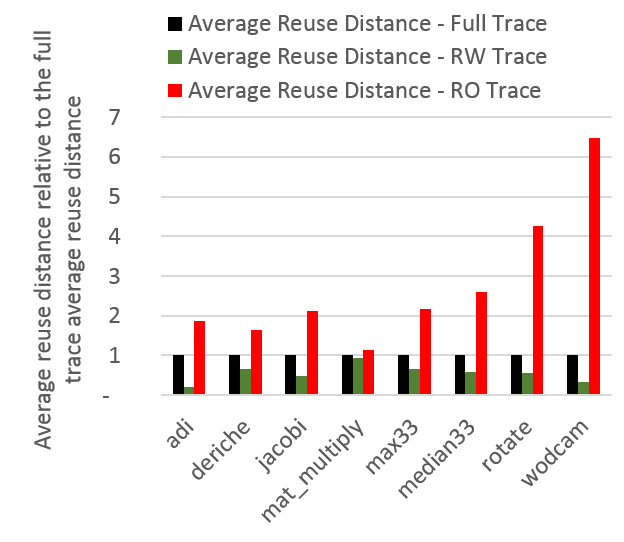
\includegraphics[width=9cm]{./images/stackdistance.png}
     \caption{Variation of the average reuse distance}
    \label{stackdistance}
\end{figure}

On all the evaluated benchmarks, two important observations can be made. First, average reuse distance of read-only data is 8.4 times bigger than the one of read-write data. Second, removing the read-only data from the main memory stream reduces the average reuse distance by 32\% in average. The read-only data present much less data locality than average data and they can create potentially more pollution into the cache hierarchy. Removing them from the main memory stream flow therefore enhances data locality of the main memory flow and leads to better cache use. This conclusion has been extended to the standard set of benchmarks Mibench~\cite{vaumourin:2014} and similar conclusions can be drawn for image and signal processing applications. 


\begin{figure}
    \centering
    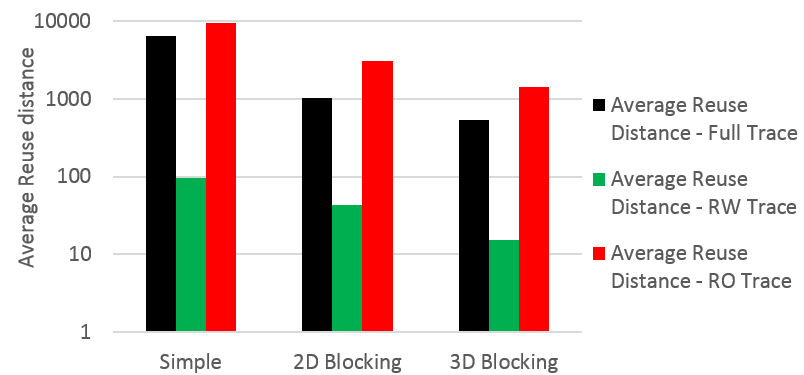
\includegraphics[width=9cm]{./images/blocking1.png}
     \caption{Average reuse distance with several tiling strategies}
    \label{blocking}
\end{figure}

\subsection{Sensitivity to code transformation}
\begin{figure}
    \centering
    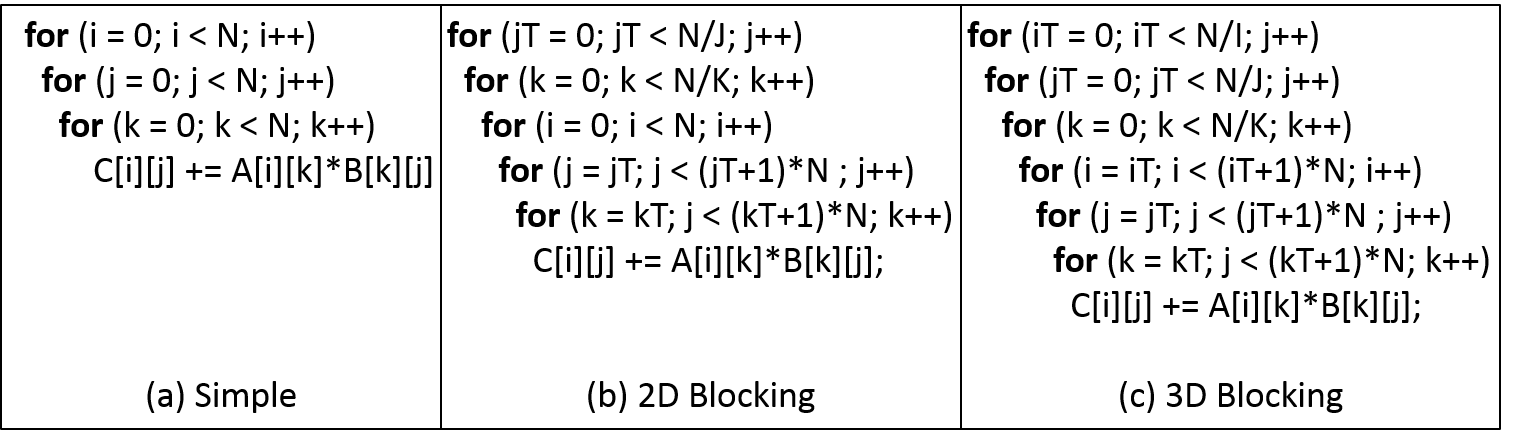
\includegraphics[width=9cm]{./images/matmul.png}
     \caption{Evaluated tiling strategies for \textit{mat\_mult}}
    \label{matmul}
\end{figure}


Read-only data detection and reuse distances depend heavily on parameters such as the degree of locality optimization applied to source code or input data sizes. As an example of locality optimization, the tiling is studied on the \textit{matrix\_multiply} benchmark. Figure \ref{matmul} shows 2D and 3D tiling transformation applied to \textit{mat\_mult} and different tile shapes are evaluated. The tile shape with the best result in terms of average reuse distance of the full trace is kept for the results of Figure \ref{blocking}. In this case, tiles parameters are K=8,J=32 for 2D tiling, and K=8,J=16,I=1 for 3D tiling. It shows that even though the average reuse distance varies with the applied transformation, the average reuse distance between the sub-memory streams remains at the same level. This locality difference comes from the algorithm structure. The read-only matrix accessed in column-order, produces long reuse distances compared to the other, tiling can reduce this distance but will always be larger than the output matrix that reuses its data between each iteration of the innner loop.  The conclusion drawn from the simple version of \textit{matrix\_multiply} stays valid with tiling transformation. However, some locality transformations such as loop fusion, can interfere with read-only data detection. For example, if a memory region is read in one loop body (creating a read-only period) and written in the other, merging the 2 loops would cancel the read-only period resulting in no detected read-only data. 

\subsection{Sensitivity to input data size}

In another direction, the influence on the results of the input data sizes has been studied. The working set size that we study stays at best one order of magnitude under classic working set size used in embedded system. However, several measure points have been taken with different input data size and they are reported Table~\ref{inputdata}. The trend of the results suggests that increasing the working set sizes increases the difference of the reuse distance illustrated Fig.~\ref{stackdistance}, reinforcing our conclusions. The illustrated difference of data locality between read-only and read-write data, motivates the idea of a specific management. The next section studies a data classification mechanism at compile-time in order to place the read-only data in the right data path. 

\begin{table}
\caption{Variation of the reuse distances relatively to input size averaged from all applications}
\label{inputdata}
\begin{tabular}{ |c|c|c|c| }
\hline
 & Avg Rd& Avg Rd & Avg Rd \\
 & Full Trace& RW Trace & RO Trace\\
\hline
Small dataset & 100\% & 60\% & 91\%\\
\hline
Large dataset&  100\% & 75\%& 291\%\\
\hline
\end{tabular}
\end{table}


\section{Read-only data Detection}

Our hardware/software co-design solution uses a static analysis inside the compiler to perform the RO/RW data classification. The great advantages of static analysis that it adds no cost on the hardware side and no execution overhead. Our solution relies on existing dataflow techniques to reach high detection rates and allows data classification at cache block granularity. 

\subsection{Static Analysis}

Our solution targets image processing applications which mainly use pointers, arrays and structures. We developed an extension of the alias analysis as an intra-procedural pass that focuses on nested computational loops. The algorithm is the following. For each loop, the pass iterates over the loop body, and maintains two lists of memory references, a read-only and a read-write list. These lists are then built for each loop nest. The results of alias analysis help us correlates the memory reference to memory regions. In order to consider a memory region as read-only, all references that points to the region must come from the read-only list. The status of memory regions can then be deduced for each loop nest and this property can vary between loop nests. The analysis uses a conservative approach in order to ensure that every reference captured is read-only. For example, if there are conditional branches in loops, the memory region needs to be read-only in all the paths in order to be considered read-only. It works the same in the loop nest is composed with several internal loops. Also, as the abstraction we use for memory regions is an interval, entire intervals are considered to be either read-only or read/write. 

So our analysis is built on top on the pointer aliasing analysis and shares the same limitation. Possible aliasing between two pointers with a different status causes a region to be conservatively considered read-write whenever the base addresses cannot proven to be disjoint. In particular, this is the case when pointers originate in parameter values instead of global or stack-allocated memory. This situation rises because production compilers like GCC tends to implement pointer aliasing analysis at function-scope in order to keep a low complexity. But in our set of applications, most of pointers are used in a different function from where they are allocated. So, we speculatively assume non-aliasing for function parameters which is true in practise for our set of applications. Run-time checks can be added in the code when this assumption is made in order to keep correct analysis with other applications. 

%Also, as we saw, some code optimization performed by the compiler can modify drastically the read-only detection so optimally, our pass would be placed at the very end of the compiler workflow. In practise however, we place our pass at the end of the list of loop analysis which is 


\begin{figure}
    \centering
    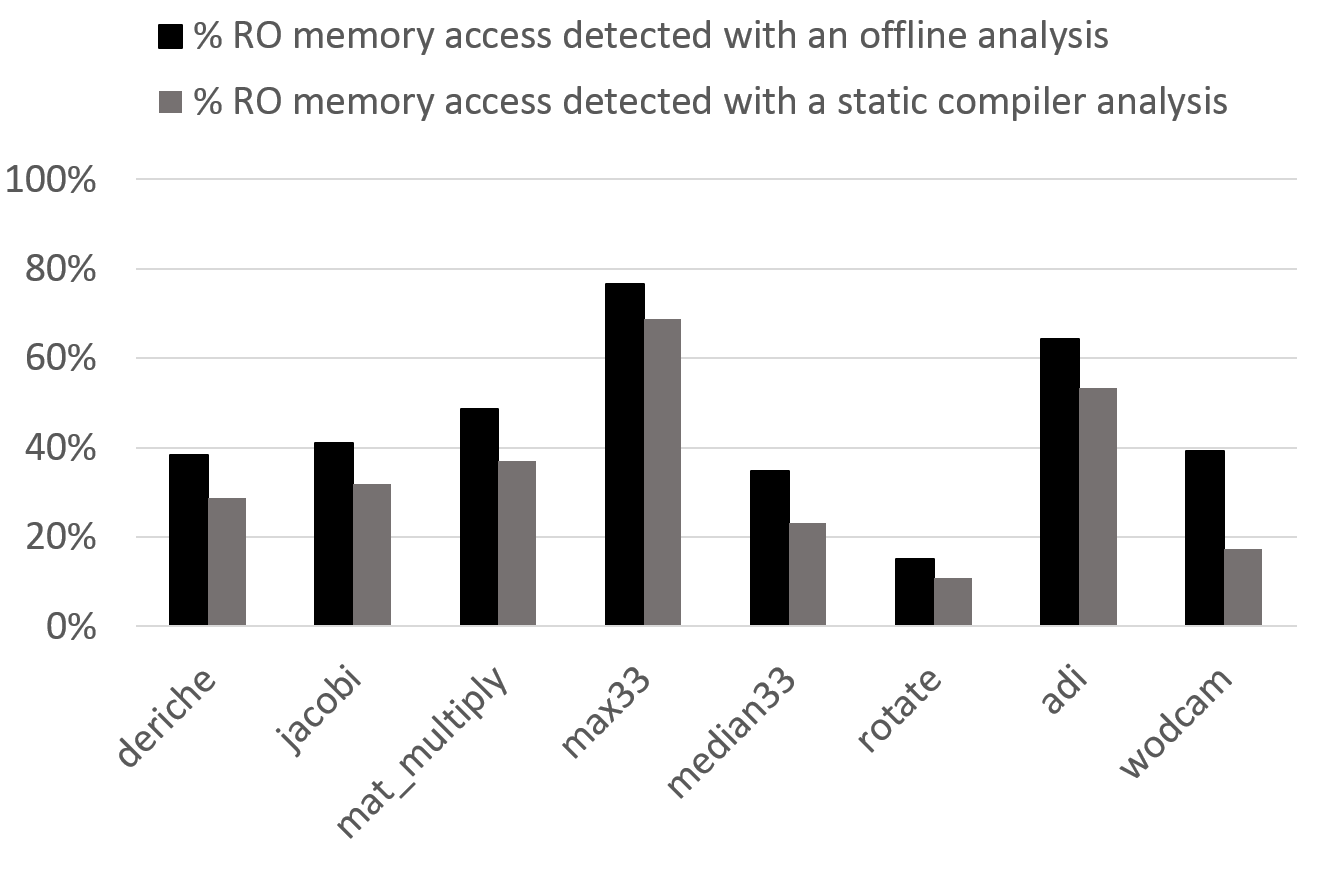
\includegraphics[width=8cm]{./images/plugin_result.png}
    \caption{Comparison between the read-only memory accesses detected with offline analysis and with the static analysis}
    \label{comparAcces}
\end{figure}

This algorithm has been implemented as a GIMPLE pass in GCC 4.9. To determine the quality of this static analysis, the results are compared to the offline analysis presented Section 3. Results in Figure ~\ref{comparAcces} show the static analysis we propose is able to capture most of the read-only memory accessed compared to the offline analysis. The detection rate is 89.7\% in average for the considered applications compared to the offline analysis, which is suitable to consider architectural specific management. 

The static analysis developed highlights the fact that read-only information is quite simple to extract at compiler level and therefore is relevant as part of a co-design architecture that proposes specific management for read-only data. 

\subsection{Compiler-Hardware Interface}

The solution assumes that each processor knows the datapath to use when accessing a given cache block. We propose to add this information directly into memory request, this technique is known as a cache collaborative technique or cache hint. Existing architectures already use these kinds of extra bits in the instruction, such as the prefetch and evict-next instruction in the Alpha 21264. We believe that, in most architectures, the increasing speed gap between memory and processor will justify the inclusion of additional bits in the instruction code in order to improve caching.

The benefits of such interface are twofold: It allows to work on block granularity classification that is proven to be important for the detection rate~\cite{Davari:2015} and it allows to transfer semantic information independent on the execution context. The information in this case is always accurate compared to prior works which exploit static information. Previous solutions use such interface to transmit locality information for data placement strategy~\cite{Beyls:2005} or dynamic cache replacement policy~\cite{Gu:2011}. However, such hints can be inaccurate because it depends on dynamic behiavor and it is hard to predict from the hardware point-of-view when the prediction made by the compiler is correct. In our proposition, since the classication is conservatively accurate, we do not need to plan for recovery mechanisms caused by classification errors. 

\section{Architecture exploration}

This section describes the architectural exploration of read-only data specific management. A dedicated cache is added along a classic cache-based memory system to handle specifically the read-only memory accesses. The exploration focuses on the design of the RO cache and the shared/private property of this cache. Starting from a generic memory hierarchy of two levels with private first level caches and shared unified last-level cache (LLC), it creates two architectural possibilities presented Figure~\ref{architecture} which describes two scenarios. Since the read-only property of the data is dynamic, data can be accessed by both data paths depending on the time of the execution. Switching technique between data paths must then be considered in order to avoid coherence issue between the read-only (RO) cache and the RW cache of the same level. The resolution of this problem can incur overheads if a cache line has to do many switches between  RO and  classic data paths because we do not consider direct transfers between caches of the same level in this work. Early studies focus on a dedicated RO Cache at L2 level. Because of the migration problem between the RW and the RO datapath, it increased the number of accesses to the main memory in a prohibitive way (up to 70\% in our study), while breaking the reuse that was happening in the L2 cache. We concluded that a dedicated L2 RO cache was not relevant and a more suitable proposition would be a cache partitionning technique between RO and RW data such as used by Khan \textit{et al.}\cite{Khan:2014}. In the following of the paper, we focus our analysis to the L1-level. 

\begin{figure}
    \centering
    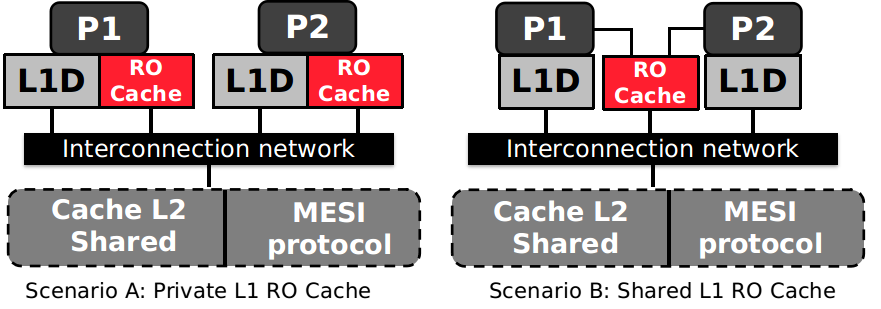
\includegraphics[width=9cm]{./images/architecture.png}
    \caption{Evaluated architecture for specific read-only data management}
    \label{architecture}
\end{figure}

\subsection{Scenario A: Private RO Cache}

The first scenario considers a private RO cache for each core. This solution is similar to the separation of the instruction cache and data cache. In this case, a cache line cannot be in the two caches so the L1D-cache and RO cache are mutually exclusive. If a cache line, present in one of the cache, needs to be accessed by the other cache, it needs first to be invalidated and eventually written back to the L2 if modified. Each entry of the sharer list in the L2 cache has an additional bit to store the location of the block (L1D or RO cache). 

\subsection{Scenario B: Shared RO Cache}

In this case, we study a RO cache shared at L1-level accross all cores. The coherence problem is resolved in this case by using the same MESI coherence state machine for RO cache as for L1D cache. From the coherence protocol point of view, it is equivalent to have a fifth L1D cache to track. Note that in our simulations, the RO cache is not multi-ported because this increases prohibitively the cost per access which is not suitable for a cache close to a processor. Instead, the requests are sequentialized and a processor may has to wait for other processors to send their request before being able to accessed the RO cache. Note that all the caches (including the RO cache) that we used are non-blocking with MSHR. Other requests can be served while a miss is pending, so it limits the stalled time on the RO cache. 

\subsection{Evaluation}

\begin{figure}
    \centering
    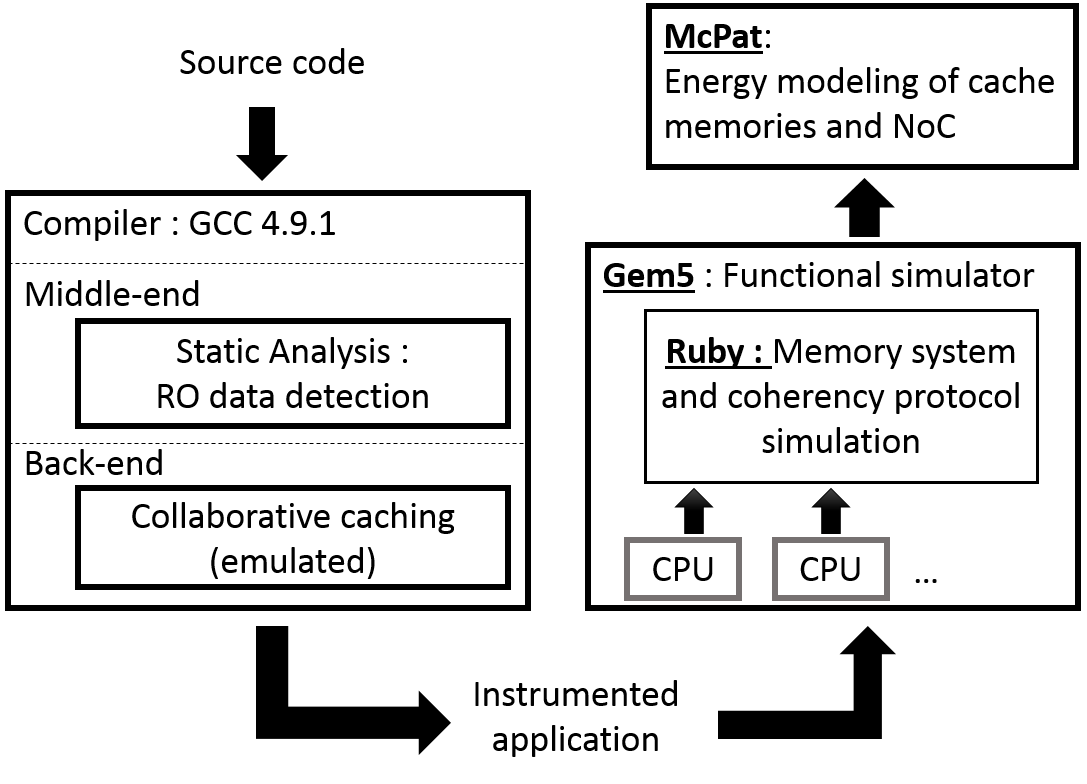
\includegraphics[width=8cm]{./images/workflow.png}
    \caption{Simulation Workflow}
    \label{workflow}
\end{figure}

For our experiments, we use the Gem5 simulator~\cite{Binkert:2011} to implement our architecture proposition, with the sub-simulator Ruby to describe the memory system and the coherence protocol. It allows detailed simulation of the cache hierarchy. The energy consumption of caches and interconnection network are obtained from the McPat framework v1.3~\cite{Li:2009}. The overall workflow is represented in Fig.~\ref{workflow} with the simulation parameters presented Table~\ref{designs}. For each scenario, we performed a design space exploration of the RO Cache and the design proposed  here is optimized for energy efficiency. 

\begin{table}
\centering
%\normalsize
\caption{Simulation parameters of the different scenarios}
\label{designs}
\begin{tabular}{ | c | c | c |}
\hline
\hline
 & L1 Data Cache& RO Cache\\
\hline
CPU & \multicolumn{2}{|c|}{4 cores in-order, 1GHz, 1 load/store unit}\\
\hline
Ref. Scenario & 32kB/64kB 2-ways & - \\
\hline
Scenario A & 32kB 2-ways & 16kB 2 ways\\
\hline
Scenario B & 32kB 2-ways  & 32KB 2-ways\\
\hline
L2 & \multicolumn{2}{|c|}{256kB 16 ways assoc.}\\
\hline
Local Network& \multicolumn{2}{|c|}{Crossbar , 64B wide, 2 cycles lat.}\\
\hline
DRAM  & \multicolumn{2}{|c|}{512MB, 1 memory channel at 12.8GB/s}\\
\hline
\hline
\end{tabular}
\end{table}

\section{Results}

\subsection{Benchmark Description}

All benchmarks are presented in Table~\ref{benchs}. They come from in-house set of benchmarks and are written in C, parallelized with OpenMP and compiled with the presented static analysis and \texttt{O3} optimization. Most of them are taken from image processing domain and no locality transformation has been used. The Fig.\ref{benchsCarac} shows the memory accesses distribution for the benchmarks. The results are produced according to the RO/RW classication scheme presented previously.

\begin{table*}
\centering
\caption{Benchmarks description}
\label{benchs}
\begin{tabular}{ |c|c|c| }
\hline
\hline
  \textbf{Benchmarks} &  \textbf{Input Data} & \textbf{Description} \\
\hline
 matrix\_multiply & 512x512 arrays&  Blocked version of matrices multiplication\\ 
\hline
 deriche & image of 1024x1024px& Canny edge detector\\
\hline
 rotate & image of 1024x1024px &  Image Rotation algorithm \\
\hline
 max33 &  image of 1024x1024px & Image blur algorithm \\
\hline
 median33 &  image of 1024x1024px& Image median algorithm\\
\hline
 jacobi & 1024x1024 matrices  & Linear equation system solver \\ 
\hline
 adi & 256 elements arrays (10 iterations) &  non-linear differential equations algorithm\\
\hline
 wodcam & 1000 test images (168x192px) &Recognition faces application based on eigenface method\\
\hline
\hline
\end{tabular}
\end{table*}


\begin{figure}
    \centering
    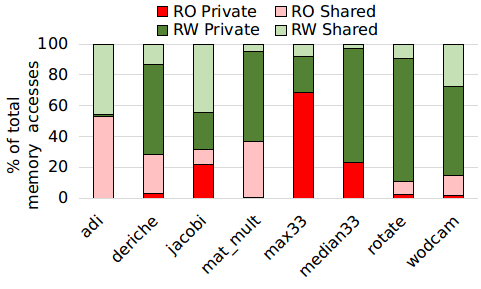
\includegraphics[width=8cm]{./images/benchs.png}
    \caption{Memory accesses classification accross benchmarks between RO/RW and Shared/Private (cache line granularity)}
    \label{benchsCarac}
\end{figure}

The main focus is the energy reduction of the system while keeping performance. The performance of the system is measured through the AMAT metric (Average Memory Access Time) because all other parameters (branch predictions, computation, ...) are constant between simulations. The energy consumption results are presented Fig.\ref{resultsConso}, the AMAT results Fig.\ref{resultsPerf} and the misses repartition at L1-level are shown in Figure~\ref{resultsMisses}, for the different scenarios. Note that the RO cache misses are counted as L1-level misses for scenarios A and B.


\begin{figure}
    \centering
    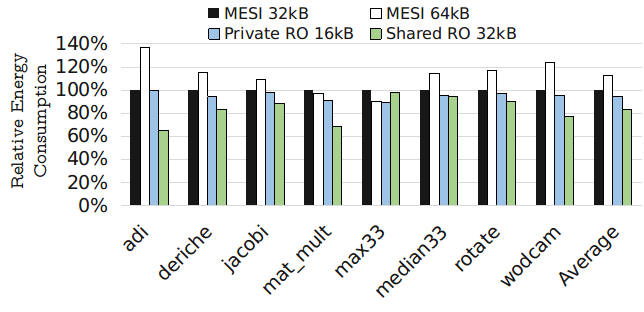
\includegraphics[width=9cm]{./images/results1.png}
    \caption{Normalized energy consumption}
    \label{resultsConso}
\end{figure}


\begin{figure}
    \centering
    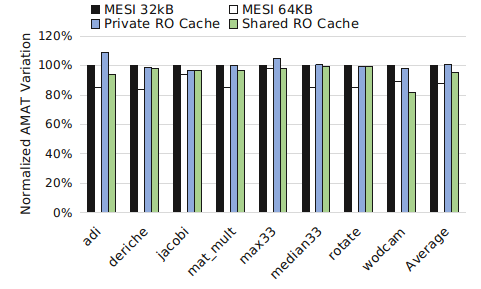
\includegraphics[width=9cm]{./images/resultsAMAT.png}
    \caption{Normalized AMAT (less is better)}
    \label{resultsPerf}
\end{figure}

\begin{figure*}
    \centering
    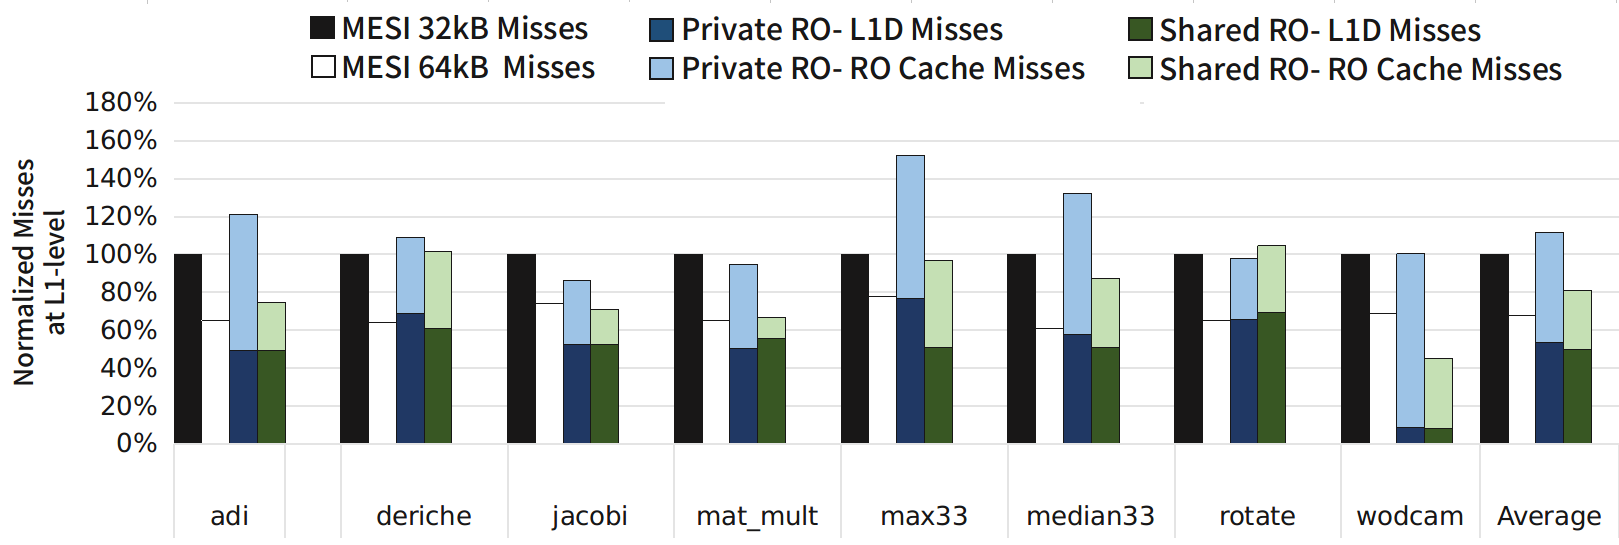
\includegraphics[width=15cm]{./images/resultsMisses1.png}
    \caption{Normalized misses at L1-level}
    \label{resultsMisses}
\end{figure*}


\subsection{Scenario A: Private RO Cache}

In scenario A, the number of cache misses stays relatively similar to the baseline even though the miss rates of L1D caches are decreased by an average of 24,2\%. As anticipated by the result of Section 3, the locality of the main memory stream is improved when the read-only data stream is removed resulting in  miss rates reduction in the L1D caches. Note that this depollution in the L1-D caches is observed in the same proportion in scenario A and B. However, for scenario A, the number of misses does not change significantly because misses occuring previously on the L1D are now being issued on the RO cache, the specific ressource allocated for the RO cache in this case is not enough to solve those misses. Read-only accesses represent only 28.5\% of the total memory access in average, and they are divided equally between the 4 cores. In this case, private read-only caches handle very few memory accesses and yet are not able to resolve misses. This negates the performance improvements on L1D-caches and points out the poor use of the RO cache resources. The small energy improvement in this proposition is based on the fact that the read-only accesses are handled in a smaller cache than the baseline, the energy cost per access is lower.

\subsection{Scenario B: Shared RO Cache}


Scenario B presents a great cache miss reduction and the best energy improvement of 16,8\% in average with a AMAT relatively constant compared to the baseline with 32kB L1D caches. Reducing misses at L1-level has a great impact on the overall memory system as it reduces also accesses to L2 cache and main memory. 


Generally speaking, sharing a cache can provoke interferences and resource conflicts. Performance degradation du to ressource conflicts here stays marginal because the RO cache handles only 28.5\% of the accesses and because the solution brings a great reduction of L1-level misses which compensates this performance degradation. Compared to the baseline with 64kB L1D caches, scenario B does not achieved a miss reduction as important but is much more energy efficient either for dynamic energy because they have a much smaller cost per access or for the leakage power because the cache used are smaller. Compared to scenario A, the depollution effect observed on the L1D caches is relatively similar. However, the difference is that some applications such as \textit{adi} and \textit{mat\_multiply} show an important miss reduction on the RO datapath because most of their read-only working set are shared. In these cases, cores are able to share the same cache block directly into the RO cache and it decreases the reuse distance of this block. Those constructive interferences are further studied with the help of the reuse distance in the next paragraph.  For other applications such as \textit{rotate}, \textit{max33} and \textit{median33} the baseline of these benchmarks is already very efficient, the miss rate is under 1\%, and it is hard for the RO cache to further increase the energy efficiency in such situation. However, the cache ressource is not wasted as in scenario A where 4 RO caches are used compared to only one in scenario B. We can see the miss rate at L1-level stays under 1\%.


\subsection{Interference analysis}

Interferences can be destructive if sharing the cache between several cores leads to a miss rate increase because cores write into cache lines currently being used by a core. It can be constructive when several cores can work on the same cache line and reduce the reuse distances of a cache line. To measure the effect of interferences that occurs in the shared RO cache between all the processors, we watch the average reuse distance of the accesses performed on the RO datapath in scenario A and B, illustrated Fig.\ref{interference}.

\begin{figure}
    \centering
    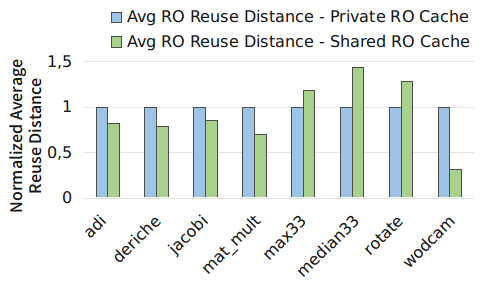
\includegraphics[width=8cm]{./images/interference.png}
    \caption{Comparison of the average Reuse distance of the RO datapath of scenario A and B}
    \label{interference}
\end{figure}

If we correlate these results with Fig.\ref{stackdistance} and Fig.\ref{resultsMisses}, it allows to understand the good results achieved  by \textit{wodcam} in our simulations. In Fig.\ref{stackdistance}, the reuse distances of the accesses performed in the read-only datapath are in average 6.3 times higher than in the RW datapath. Most of the misses come from the read-only data path in this case (Fig.\ref{resultsMisses}, and by sharing the RO cache accross all cores, Fig.\ref{interference} points at the important constructive interferences that occurs in the RO datapath improving the RO data locality. This locality improvement is translated into an important miss reduction in the RO cache for \textit{wodcam}. This effect can also be observed for \textit{adi} and \textit{mat\_multiply} in a less significant manner. Note that locality improvement that not always translated into miss reduction such as in \textit{jacobi} as reuse distances need to be reduced enough to fit into the RO cache. Constructive interference is a fine-grain phenomena hard to achieve as it depends on the execution speed of the threads but can improve significantly the locality. Scenario B is the best for energy improvement and further analysis on this scenario is performed in the following sections.

%In our simulations, constructive interferences could only happen when RO shared data are present in the working set. As shown in Fig.\ref{benchsCarac}, for \textit{max33} and  \textit{median33}, the RO working set is private and interferences can be only destructives in this case. But it stays a better solution than scenario A as the cache ressources are not wasted and destructive interferences 

\subsection{Impact of the RO cache latency}

During the previous simulations, the RO cache is configured to have the same latency as a classical L1-D cache because they are logically on the same level. In a real system, the RO cache latency is expected to be higher as the RO cache is shared across cores. Moreover, the latency of the RO cache is more critical as it can potentially stall all processors. Some additional experiments have been made in order to study the impact of the latency of the RO cache on the overall system performance. This latency have been varied from 3 cycles to 15 cycles and the AMAT of the system compared to the baseline architecture (L1D of 32kB) is shown Fig\ref{rolatency}. As a reminder, the latency of an L1D-cache is 3 cycles, for L2 cache, 15 cycles. For a latency of 5 cycles, there is no performance degradation compared to the baseline architecture. The 5\% degradation barrier is crossed with a RO latency of 9 cycles. Even though the variation is linear, the sensibility is not the same for every application. The sensibility to the RO datapath can be explained mostly by the numbers of requests handled. For example, \textit{max33} is more sensitive than \textit{rotate} to this parameter because the proportion of total CPU fetches handled through the RO cache is respectively 68\% and 11\%. These results show that there is no performance degradation for a large range of RO cache latencies.

\begin{figure}
    \centering
    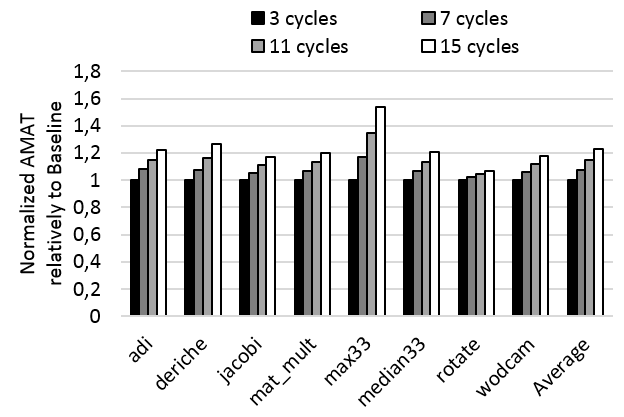
\includegraphics[width=9cm]{./images/rolatency.png}
    \caption{Sensitivity of the AMAT relatively to the RO cache latency}
    \label{rolatency}
\end{figure}


\subsection{Scalability of the solution}
\begin{figure}
    \centering
    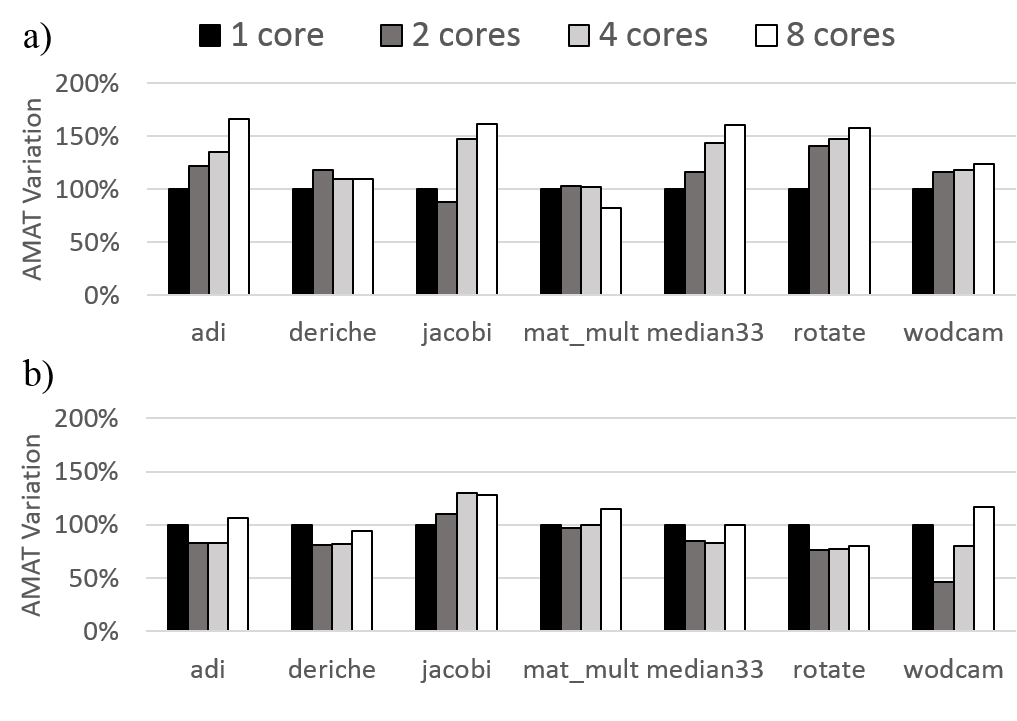
\includegraphics[width=9cm]{./images/scalabilityAMAT.png}
    \caption{For scenario B, AMAT variation of a) the RW datapath (L1D-L2) and b) RO datapath (Cache RO-L2) normalized to the unicore baseline}
    \label{amatVariation}
\end{figure}

We study the results of Scenario B regarding the strong scalability of the memory system. Figure \ref{amatVariation} shows the average AMAT for the two datapaths, normalized to the baseline unicore solution. As the number of cores increases, bank conflicts, contention on shared ressources (bandwidth and caches) and coherence protocol may impact performance of any of the datapath (RO and RW). Figure \ref{amatVariation} shows that the response time of the RW data path is essentially impacted by these destructive interferences. On the contrary, for the RO datapath, the AMAT stays relatively stable because increasing the number of cores increases the cache sharing effect, outbalancing the previous negative impacts. As the applications are parallelized with OpenMP and threads run on identical processors, threads run similar codes at the same IPC, so they tend to work on shared data at the same moment of the execution allowing reuse accross processors into the RO cache.

 
\section{Specific RO Cache optimization}

Adding more caches to the memory system increases the design complexity but also opens degrees of freedom for specific optimizations. This section explores one possible specific optimization for the RO cache based on the observation that it issues only read requests. This property is guaranteed by the conservative static analysis. No tracking is then needed from the coherence protocol in the same way as instruction cache. Such optimization is related to an important number of work from the literature proposing to reduce the impact of coherence by limiting expensive coherence mechanisms to shared read-write cache blocks. Several recent propositions~\cite{Cuesta:2013}\cite{Ros:2012}\cite{Davari:2015} classify data as private or read-only in order to reduce the coherence overhead and reduce directory design, this classification is done mostly at OS or hardware level. Such propositions are shown to improve the scalability of the architecture and reduce the energy consumption. Such solutions initialize all data status as private. When shared write accesses occurs, the status of the data (a whole page or a cache block depending on the solution) switches to shared and costly coherence recovery mechanisms are used to recover from this classification error. Moreover, such solutions usually do not consider transition back to the private status. Compared to such solutions, our proposition allows the status transitions of the cache block and does not need additional harware mechanism to protect against classification error as the compiler garantees the correctness of the classification. Our proposition of a shared read-only cache at the first level of hierarchy contributes to an orthogonal approach to such optimization. So, it could include read-write data that present read-only periods into this optimization, increasing the scope of such optimization.\\

The coherence state machine of the RO and L2 cache controller have
been modified in order to avoid the tracking of the read-only cache
blocks. The state machine of the read-only cache is very similar to an
L1D cache in a unicore system. Figure~\ref{incoherent} illustrates two
examples that benefit from a non coherent RO cache. In the first case,
a read request incurs a miss in the cache and a cache block needs to
be invalidated. The L1D cache has to inform the L2 cache about this
eviction even if the cache block is not modified, so that the L2
controller can update the sharers list. This property is required in
order to keep the system inclusive. This precaution is not needed with
the RO cache, resulting into several benefits. First, evictions from
the RO cache need less messages. Second, the system is not fully
inclusive anymore, as cache block can be evicted from the L2 cache and
kept into the RO cache without specific tracking, increasing
cache efficiency. The second example illustrates the fact that RO
cache operations do not change coherence state of the others
caches. Usually, a read request of a cache block that is already
modified in another L1D cache creates a costly downgrade transaction
of the cache block from Modified to Shared. With a RO cache, such
transaction requires less messages and no modification of the
coherence state of the cache block in the L1D and L2 caches. It means
that the L1D cache still has read/write permission to the cache block
after a read access from the RO cache, and potentially a future write
request will not miss.


The state machine of a non coherent RO cache has been implemented into Gem5 and compared to the result with the coherent RO cache. As anticipated with the examples of Figure~\ref{resultIncoherent}, a non coherent RO cache mainly reduces the network traffic of 26\% compared to coherent RO cache, decreasing the energy consumption by 4\% in average compared to the results of the previous section. It can also
prevent the prohibitive increase of messages that occur for example on
\textit{median33} and \textit{max33} due to the L1 miss
increase observed for these applications with scenario B. But cache
efficiency stays relatively stable between the two scenarios. On the
evaluated applications, only \textit{adi} presents an important amount
of Modified->Shared transitions on L1D caches that benefit from the
non coherent read-only cache, in the same way as the situation
described in the latter case of Figure~\ref{incoherent}. For
\textit{adi}, cache efficiency is improved and significant gain on the
AMAT (17,6\%) and energy consumption (11,3\%) can be found compared a
solution with a coherent RO cache.

\begin{figure}
    \centering
    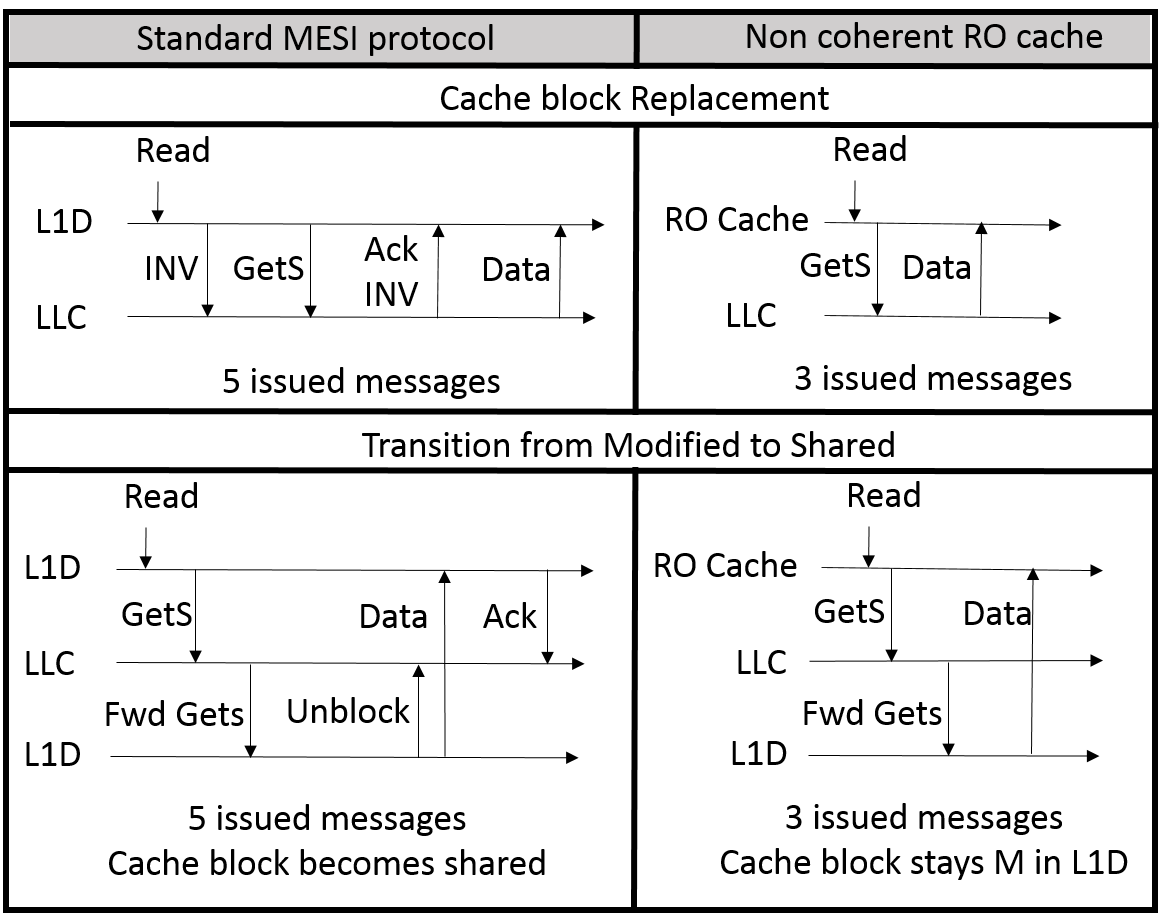
\includegraphics[width=9cm]{./images/incoherent.png}
    \caption{Difference of the procedure with non coherent RO cache during  cache block remplacement and downgrading operation}
    \label{incoherent}
\end{figure}


\begin{figure}
    \centering
    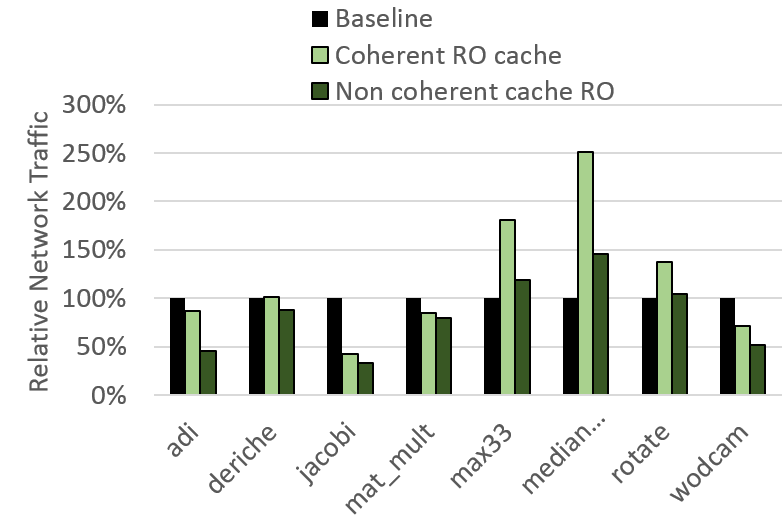
\includegraphics[width=9cm]{./images/resultIncoherent.png}
    \caption{Network traffic variation for coherent and non coherent RO cache}
    \label{resultIncoherent}
\end{figure}


\section{Conclusion}

With the end of the CMOS scalability, a new way to improve the efficiency of cache-based memory system is to propose heterogeneous management. In this paper the feasibility and benefits of a specific management of read-only data in the memory organization is studied. A complete hardware/software codesign is proposed, making the solution transparent to the user while achieving significant energy improvements, with no performance degradation. This separation increases the cache efficiency of the system, and allows specific optimizations for the read-only cache. We have shown that this architectural modification follows the scalability of the shared caches and can be further improved if using non-coherent RO caches. The proposed solution has been validated on a set of image processing applications, but the same methodology could be extended to a larger set of applications. 

\bibliographystyle{ACM-Reference-Format}
\bibliography{cases} 

\end{document}
